\documentclass{article}
\usepackage{cmap}
\usepackage[utf8]{inputenc}
\usepackage[english,ukrainian]{babel}
\usepackage{graphicx}
\usepackage{geometry}
\usepackage{listings}
\usepackage{amsmath}
\usepackage{float}
\geometry{
	a4paper,
	left=20mm,
	right=20mm,
	top=20mm,
	bottom=20mm
}
\lstset{
	language=c++,
	tabsize=4,
	keepspaces,
	showstringspaces=false,
	breaklines,
}
\graphicspath{ {./pictures} }
\setlength{\parindent}{4em}

\newcommand\subject{Операційні системи}
\newcommand\lecturer{старший викладач кафедри ПЗ\\Грицай О.Д.}
\newcommand\teacher{старший викладач кафедри ПЗ\\Грицай О.Д.}
\newcommand\mygroup{ПЗ-22}
\newcommand\lab{9}
\newcommand\theme{Організація взаємодії між процесами}
\newcommand\purpose{Ознайомитися зі способами міжпроцесної взаємодії. Ознайомитися з
	класичним прикладом взаємодії між процесами на прикладі задачі «виробник –
	споживач». Навчитися працювати із процесами з використанням способів
	міжпроцесної взаємодії, синхронізувати їхню роботу}

\begin{document}
\begin{normalsize}
	\begin{titlepage}
		\thispagestyle{empty}
		\begin{center}
			\textbf{МІНІСТЕРСТВО ОСВІТИ І НАУКИ УКРАЇНИ\\
				НАЦІОНАЛЬНИЙ УНІВЕРСИТЕТ "ЛЬВІВСЬКА ПОЛІТЕХНІКА"}
		\end{center}
		\begin{flushright}
			Інститут \textbf{КНІТ}\\
			Кафедра \textbf{ПЗ}
		\end{flushright}
		\vspace{200pt}
		\begin{center}
			\textbf{ЗВІТ}\\
			\vspace{10pt}
			До лабораторної роботи № \lab\\
			\textbf{На тему}: “\textit{\theme}”\\
			\textbf{З дисципліни}: “\subject”
		\end{center}
		\vspace{112pt}
		\begin{flushright}
			
			\textbf{Лектор}:\\
			\lecturer\\
			\vspace{28pt}
			\textbf{Виконав}:\\
			
			студент групи \mygroup\\
			Коваленко Д.М.\\
			\vspace{28pt}
			\textbf{Прийняла}:\\
			
			\teacher\\
			
			\vspace{28pt}
			«\rule{1cm}{0.15mm}» \rule{1.5cm}{0.15mm} 2022 р.\\
			$\sum$ = \rule{1cm}{0.15mm}……………\\
			
		\end{flushright}
		\vspace{\fill}
		\begin{center}
			\textbf{Львів — 2022}
		\end{center}
	\end{titlepage}
		
	\begin{description}
		\item[Тема.] \theme.
		\item[Мета.] \purpose.
	\end{description}

	\section*{Лабораторне завдання}
	
	\begin{figure}[H]
		\centering
		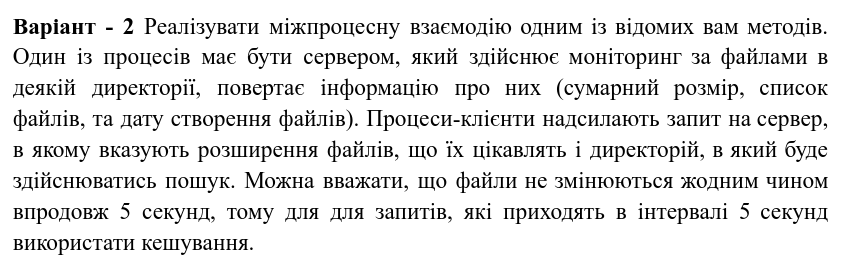
\includegraphics[scale=0.5]{v}
	\end{figure}

	\section*{Хід роботи}	
	\section*{WINDOWS}
	\textbf{main.cpp}
	\begin{lstlisting}
#include <unistd.h>
#include "mainwindow.h"
#include "ui_mainwindow.h"
#include <iostream>
#include <QFileDialog>
#include <stdio.h>
#include <stdlib.h>
#include <fcntl.h>
#include "random"

using namespace std;

MainWindow::MainWindow(QWidget *parent)
: QMainWindow(parent)
, ui(new Ui::MainWindow)
{
	ui->setupUi(this);
	ui->tableWidget->setColumnWidth(0, 50);
	srand(time(NULL));
}

MainWindow::~MainWindow()
{
	delete ui;
}

class MyException : public exception
{
	string _msg;
	public:
	MyException(string msg) : _msg(msg) {}
	
	virtual const char* what() const noexcept override
	{
		return _msg.c_str();
	}
};

void MainWindow::on_pushButton_clicked()
{
	QString dir = QFileDialog::getExistingDirectory(this, "Monitor directory", QString(), QFileDialog::ShowDirsOnly);
	ui->textEdit_directories->setText(ui->textEdit_directories->toPlainText() + dir + '\n');
}

void MainWindow::on_pushButton_Find_clicked()
{
	//forming the request
	int myId = rand();
	QString request = QString::number(myId) + separator;
	QStringList dirList = ui->textEdit_directories->toPlainText().split("\n");
	QStringList extList = ui->textEdit_extentions->toPlainText().split("\n");
	
	for(auto dir = dirList.cbegin(); dir != dirList.cend(); dir++)
	{
		if(!dir->isEmpty())
		{
			request += *dir + ',';
		}
	}
	if(request.back() == ',')
	{
		request.back() = separator;
	}
	else
	{
		request += separator;
	}
	
	for(auto ext = extList.cbegin(); ext != extList.cend(); ext++)
	{
		if(!ext->isEmpty())
		{
			request += *ext + ',';
		}
	}
	if(request.back() == ',')
	{
		request.back() = '\n';
	}
	else
	{
		request += '\n';
	}
	
	qDebug() << "Request is: " << request;
	
	//Outputting the requests
	struct flock olock;
	olock.l_type = F_WRLCK;
	olock.l_whence = SEEK_SET;
	olock.l_start = 0;
	olock.l_len = 0;
	
	int ofd;
	while ((ofd = open(requestFilePath.c_str(), O_WRONLY | O_APPEND, 0666)) < 0) {
		creat(requestFilePath.c_str(), 0666);
	};
	
	while (fcntl(ofd, F_SETLK, &olock) < 0);
	
	write(ofd, request.toStdString().c_str(), strlen(request.toStdString().c_str()));
	qDebug() << "Something is written to req file";
	
	olock.l_type = F_UNLCK;
	while (fcntl(ofd, F_SETLK, &olock) < 0);
	
	//Reading the responses
	struct flock ilock;
	ilock.l_type = F_RDLCK;
	ilock.l_whence = SEEK_SET;
	ilock.l_start = 0;
	ilock.l_len = 0;
	
	int ifd;
	while ((ifd = open(responseFilePath.c_str(), O_RDWR | O_APPEND, 0666)) < 0);
	
	int bufferSize = 4096;
	char buffer[bufferSize];
	
	QList<QString> requiredResponses = QList<QString>();
	
	while(requiredResponses.isEmpty()) {
		ilock.l_type = F_RDLCK;
		while (fcntl(ifd, F_SETLK, &ilock) < 0);
		
		while(read(ifd, &buffer, bufferSize) > 0);
		
		std::string input = std::string(buffer, 0, bufferSize);
		
		qDebug() << "Readings: " << buffer;
		
		QList<QString> responses = QString::fromStdString(input).split('\n');
		
		qDebug() << "Responses: " << responses;
		
		requiredResponses = filterIfContains(responses, QString::number(myId));
		
		qDebug() << "Required responses (" << QString::number(myId) << "): " << requiredResponses;
		
		ilock.l_type = F_UNLCK;
		while (fcntl(ifd, F_SETLK, &ilock) < 0);
		
		sleep(3);
	}
	
	
	//    QList<QString> otherResponses = filterIfNotContains(responses, QString::number(myId));
	
	//    ilock.l_type = F_WRLCK;
	//    while (fcntl(ifd, F_SETLK, &ilock) < 0);
	
	//    while ((ifd = open(responseFilePath.c_str(), O_RDWR | O_TRUNC, 0666)) < 0);
	
	//    for (QString element : otherResponses) {
		//        std::string responseString = element.toStdString() + "\n";
		
		//        write(ifd, responseString.c_str(), strlen(responseString.c_str()));
		//    }
	
	ilock.l_type = F_UNLCK;
	while (fcntl(ifd, F_SETLK, &ilock) < 0);
	
	qDebug() << "cock 1";
	
	//penis
	
	if (!requiredResponses.isEmpty()) {
		QStringList list = requiredResponses[0].split(separator);
		QString generalSize = list[1];
		ui->statusbar->showMessage("  General size: " + generalSize, 0);
		
		if(list.size() < 3) {
			throw MyException("Files in this directories are not found");
		}
		
		ui->tableWidget->clearContents();
		QList<QString> entries = list[2].split(iseparator);
		for(int i = 0; i < entries.size(); i++) {
			QStringList subList = entries[i].split(',');
			QString fileName = subList[0];
			QString fileBirth = subList[1];
			
			ui->tableWidget->insertRow(i);
			ui->tableWidget->setItem(i, 0, new QTableWidgetItem(QString::number(i + 1)));
			ui->tableWidget->item(i, 0)->setTextAlignment(Qt::AlignCenter);
			ui->tableWidget->setItem(i, 1, new QTableWidgetItem(fileName));
			ui->tableWidget->setItem(i, 2, new QTableWidgetItem(fileBirth));
		}
	}
}

QList<QString> MainWindow::filterIfContains(QList<QString> origin, QString sample) {
	QList<QString> results = QList<QString>();
	
	for (QString element : origin) {
		if (element.contains(sample)) {
			results.append(element);
		}
	}
	
	return results;
}

QList<QString> MainWindow::filterIfNotContains(QList<QString> origin, QString sample) {
	QList<QString> results = QList<QString>();
	
	for (QString element : origin) {
		if (!element.contains(sample)) {
			results.append(element);
		}
	}
	
	return results;
}


	\end{lstlisting}
	
	\begin{figure}[H]
		\centering
		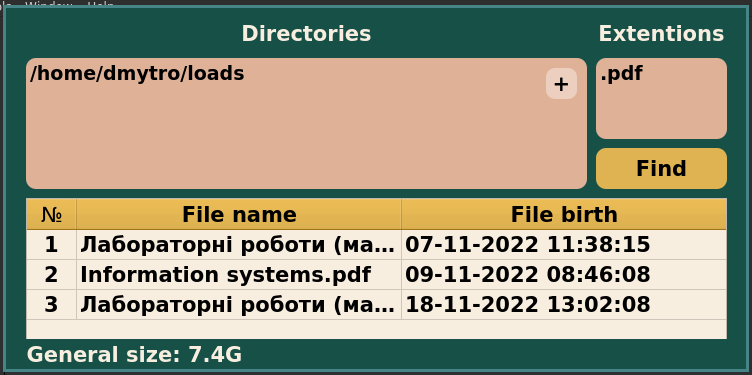
\includegraphics[scale=0.6]{1}
		\caption{Виконання програми windows}
	\end{figure}

\section*{LINUX}
\textbf{main.cpp}
\begin{lstlisting}
#include "mainwindow.h"
#include "ui_mainwindow.h"
#include "server.h"
#include "qdebug.h"
#include <unistd.h>
#include "mainwindow.h"
#include "ui_mainwindow.h"
#include <iostream>
#include <QFileDialog>
#include <stdio.h>
#include <stdlib.h>
#include <fcntl.h>

MainWindow::MainWindow(QWidget *parent)
: QMainWindow(parent)
, ui(new Ui::MainWindow)
{
	ui->setupUi(this);
}

MainWindow::~MainWindow() {
	delete ui;
}

void MainWindow::on_pushButton_clicked() {
	Server * server = new Server();
	
	QList<int> proccessedRequests = QList<int>();
	
	while(1) {
		//Reading the requests
		struct flock ilock;
		ilock.l_type = F_RDLCK;
		ilock.l_whence = SEEK_SET;
		ilock.l_start = 0;
		ilock.l_len = 0;
		
		int ifd;
		while ((ifd = open(requestFilePath.c_str(), O_RDWR | O_APPEND, 0666)) < 0);
		
		while (fcntl(ifd, F_SETLK, &ilock) < 0);
		
		int bufferSize = 4096;
		char buffer[bufferSize];
		
		while(read(ifd, &buffer, bufferSize) > 0);
		
		std::string input = std::string(buffer, 0, bufferSize);
		
		qDebug() << "Readings: " << buffer;
		
		ilock.l_type = F_UNLCK;
		while (fcntl(ifd, F_SETLK, &ilock) < 0);
		
		//1804289383@/home/piktur/OSLab9Server@.cpp
		QList<QString> requests = QString::fromStdString(input).split('\n');
		requests = filterIfNotContains(requests, proccessedRequests);
		
		if (requests.size() > 0) requests.pop_back();
		
		qDebug() << "Requests: " << requests;
		if (requests.size() > 0) {
			//Outputting the responses
			struct flock olock;
			olock.l_type = F_WRLCK;
			olock.l_whence = SEEK_SET;
			olock.l_start = 0;
			olock.l_len = 0;
			
			int ofd;
			while ((ofd = open(responseFilePath.c_str(), O_RDWR | O_APPEND, 0666)) < 0) {
				creat(responseFilePath.c_str(), 0666);
			};
			
			while (fcntl(ofd, F_SETLK, &olock) < 0);
			
			for (QString request : requests) {
				server->request(request);
				
				Response* response;
				while (!(response = server->response()));
				
				std::string responseString = response->toString().toStdString();
				responseString.pop_back();
				responseString += "\n";
				
				qDebug() << "Response: " << response->toString();
				
				write(ofd, responseString.c_str(), strlen(responseString.c_str()));
				
				qDebug() << "Something is written to resp file";
				
				proccessedRequests.append(request.split(separator)[0].toInt());
			}
			
			olock.l_type = F_UNLCK;
			while (fcntl(ofd, F_SETLK, &olock) < 0);
		}
		
		sleep(3);
	}
}

QList<QString> MainWindow::filterIfContains(QList<QString> origin, QList<int> ids) {
	if (ids.isEmpty()) return origin;
	
	QList<QString> results = QList<QString>();
	
	for (QString element : origin) {
		bool condition = true;
		for (int id : ids) {
			if (!element.contains(QString::number(id))) {
				condition = false;
			}
		}
		if (condition) results.append(element);
	}
	
	return results;
}

QList<QString> MainWindow::filterIfNotContains(QList<QString> origin, QList<int> ids) {
	if (ids.isEmpty()) return origin;
	
	QList<QString> results = QList<QString>();
	
	for (QString element : origin) {
		bool condition = true;
		for (int id : ids) {
			if (element.contains(QString::number(id))) {
				condition = false;
			}
		}
		if (condition) results.append(element);
	}
	
	return results;
}

}
\end{lstlisting}
	
	\section*{Висновок}
	Під час виконання лабораторної роботи я ознайомився зі способами міжпроцесної взаємодії. Ознайомився з
	класичним прикладом взаємодії між процесами на прикладі задачі «виробник –
	споживач». Навчився працювати із процесами з використанням способів
	міжпроцесної взаємодії, синхронізував їхню роботу.
	
	 
\end{normalsize}
\end{document}
